\documentclass[nofonts,]{tufte-handout}

% ams
\usepackage{amssymb,amsmath}

\usepackage{ifxetex,ifluatex}
\usepackage{fixltx2e} % provides \textsubscript
\ifnum 0\ifxetex 1\fi\ifluatex 1\fi=0 % if pdftex
  \usepackage[T1]{fontenc}
  \usepackage[utf8]{inputenc}
\else % if luatex or xelatex
  \makeatletter
  \@ifpackageloaded{fontspec}{}{\usepackage{fontspec}}
  \makeatother
  \defaultfontfeatures{Ligatures=TeX,Scale=MatchLowercase}
  \makeatletter
  \@ifpackageloaded{soul}{
     \renewcommand\allcapsspacing[1]{{\addfontfeature{LetterSpace=15}#1}}
     \renewcommand\smallcapsspacing[1]{{\addfontfeature{LetterSpace=10}#1}}
   }{}
  \makeatother
\fi

% graphix
\usepackage{graphicx}
\setkeys{Gin}{width=\linewidth,totalheight=\textheight,keepaspectratio}

% booktabs
\usepackage{booktabs}

% url
\usepackage{url}

% hyperref
\usepackage{hyperref}

% units.
\usepackage{units}


\setcounter{secnumdepth}{2}

% citations
\usepackage{natbib}
\bibliographystyle{plainnat}

%% tint override
\setcitestyle{round} 

% pandoc syntax highlighting
\usepackage{color}
\usepackage{fancyvrb}
\newcommand{\VerbBar}{|}
\newcommand{\VERB}{\Verb[commandchars=\\\{\}]}
\DefineVerbatimEnvironment{Highlighting}{Verbatim}{commandchars=\\\{\}}
% Add ',fontsize=\small' for more characters per line
\newenvironment{Shaded}{}{}
\newcommand{\AlertTok}[1]{\textcolor[rgb]{1.00,0.00,0.00}{#1}}
\newcommand{\AnnotationTok}[1]{\textcolor[rgb]{0.00,0.50,0.00}{#1}}
\newcommand{\AttributeTok}[1]{#1}
\newcommand{\BaseNTok}[1]{#1}
\newcommand{\BuiltInTok}[1]{#1}
\newcommand{\CharTok}[1]{\textcolor[rgb]{0.00,0.50,0.50}{#1}}
\newcommand{\CommentTok}[1]{\textcolor[rgb]{0.00,0.50,0.00}{#1}}
\newcommand{\CommentVarTok}[1]{\textcolor[rgb]{0.00,0.50,0.00}{#1}}
\newcommand{\ConstantTok}[1]{#1}
\newcommand{\ControlFlowTok}[1]{\textcolor[rgb]{0.00,0.00,1.00}{#1}}
\newcommand{\DataTypeTok}[1]{#1}
\newcommand{\DecValTok}[1]{#1}
\newcommand{\DocumentationTok}[1]{\textcolor[rgb]{0.00,0.50,0.00}{#1}}
\newcommand{\ErrorTok}[1]{\textcolor[rgb]{1.00,0.00,0.00}{\textbf{#1}}}
\newcommand{\ExtensionTok}[1]{#1}
\newcommand{\FloatTok}[1]{#1}
\newcommand{\FunctionTok}[1]{#1}
\newcommand{\ImportTok}[1]{#1}
\newcommand{\InformationTok}[1]{\textcolor[rgb]{0.00,0.50,0.00}{#1}}
\newcommand{\KeywordTok}[1]{\textcolor[rgb]{0.00,0.00,1.00}{#1}}
\newcommand{\NormalTok}[1]{#1}
\newcommand{\OperatorTok}[1]{#1}
\newcommand{\OtherTok}[1]{\textcolor[rgb]{1.00,0.25,0.00}{#1}}
\newcommand{\PreprocessorTok}[1]{\textcolor[rgb]{1.00,0.25,0.00}{#1}}
\newcommand{\RegionMarkerTok}[1]{#1}
\newcommand{\SpecialCharTok}[1]{\textcolor[rgb]{0.00,0.50,0.50}{#1}}
\newcommand{\SpecialStringTok}[1]{\textcolor[rgb]{0.00,0.50,0.50}{#1}}
\newcommand{\StringTok}[1]{\textcolor[rgb]{0.00,0.50,0.50}{#1}}
\newcommand{\VariableTok}[1]{#1}
\newcommand{\VerbatimStringTok}[1]{\textcolor[rgb]{0.00,0.50,0.50}{#1}}
\newcommand{\WarningTok}[1]{\textcolor[rgb]{0.00,0.50,0.00}{\textbf{#1}}}

% longtable

% multiplecol
\usepackage{multicol}

% strikeout
\usepackage[normalem]{ulem}

% morefloats
\usepackage{morefloats}


% tightlist macro required by pandoc >= 1.14
\providecommand{\tightlist}{%
  \setlength{\itemsep}{0pt}\setlength{\parskip}{0pt}}

% title / author / date
\title{Bar Charts in ggplot With Multiple Outcomes}
\author{Andy Grogan-Kaylor}
\date{2022-03-07}

%% -- tint overrides
%% fonts, using roboto (condensed) as default
\usepackage[sfdefault,condensed]{roboto}
%% also nice: \usepackage[default]{lato}

%% colored links, setting 'borrowed' from RJournal.sty with 'Thanks, Achim!'
\RequirePackage{color}
\definecolor{link}{rgb}{0.1,0.1,0.8} %% blue with some grey
\hypersetup{
  colorlinks,%
  citecolor=link,%
  filecolor=link,%
  linkcolor=link,%
  urlcolor=link
}

%% macros
\makeatletter

%% -- tint does not use italics or allcaps in title
\renewcommand{\maketitle}{%     
  \newpage
  \global\@topnum\z@% prevent floats from being placed at the top of the page
  \begingroup
    \setlength{\parindent}{0pt}%
    \setlength{\parskip}{4pt}%
    \let\@@title\@empty
    \let\@@author\@empty
    \let\@@date\@empty
    \ifthenelse{\boolean{@tufte@sfsidenotes}}{%
      %\gdef\@@title{\sffamily\LARGE\allcaps{\@title}\par}%
      %\gdef\@@author{\sffamily\Large\allcaps{\@author}\par}%
      %\gdef\@@date{\sffamily\Large\allcaps{\@date}\par}%
      \gdef\@@title{\begingroup\fontseries{b}\selectfont\LARGE{\@title}\par}%
      \gdef\@@author{\begingroup\fontseries{l}\selectfont\Large{\@author}\par}%
      \gdef\@@date{\begingroup\fontseries{l}\selectfont\Large{\@date}\par}%
    }{%
      %\gdef\@@title{\LARGE\itshape\@title\par}%
      %\gdef\@@author{\Large\itshape\@author\par}%
      %\gdef\@@date{\Large\itshape\@date\par}%
      \gdef\@@title{\begingroup\fontseries{b}\selectfont\LARGE\@title\par\endgroup}%
      \gdef\@@author{\begingroup\fontseries{l}\selectfont\Large\@author\par\endgroup}%
      \gdef\@@date{\begingroup\fontseries{l}\selectfont\Large\@date\par\endgroup}%
    }%
    \@@title
    \@@author
    \@@date
  \endgroup
  \thispagestyle{plain}% suppress the running head
  \tuftebreak% add some space before the text begins
  \@afterindentfalse\@afterheading% suppress indentation of the next paragraph
}

%% -- tint does not use italics or allcaps in section/subsection/paragraph
\titleformat{\section}%
  [hang]% shape
  %{\normalfont\Large\itshape}% format applied to label+text
  {\fontseries{b}\selectfont\Large}% format applied to label+text
  {\thesection}% label
  {1em}% horizontal separation between label and title body
  {}% before the title body
  []% after the title body

\titleformat{\subsection}%
  [hang]% shape
  %{\normalfont\large\itshape}% format applied to label+text
  {\fontseries{m}\selectfont\large}% format applied to label+text
  {\thesubsection}% label
  {1em}% horizontal separation between label and title body
  {}% before the title body
  []% after the title body

\titleformat{\paragraph}%
  [runin]% shape
  %{\normalfont\itshape}% format applied to label+text
  {\fontseries{l}\selectfont}% format applied to label+text
  {\theparagraph}% label
  {1em}% horizontal separation between label and title body
  {}% before the title body
  []% after the title body

%% -- tint does not use italics here either
% Formatting for main TOC (printed in front matter)
% {section} [left] {above} {before w/label} {before w/o label} {filler + page} [after]
\ifthenelse{\boolean{@tufte@toc}}{%
  \titlecontents{part}% FIXME
    [0em] % distance from left margin
    %{\vspace{1.5\baselineskip}\begin{fullwidth}\LARGE\rmfamily\itshape} % above (global formatting of entry)
    {\vspace{1.5\baselineskip}\begin{fullwidth}\fontseries{m}\selectfont\LARGE} % above (global formatting of entry)
    {\contentslabel{2em}} % before w/label (label = ``II'')
    {} % before w/o label
    {\rmfamily\upshape\qquad\thecontentspage} % filler + page (leaders and page num)
    [\end{fullwidth}] % after
  \titlecontents{chapter}%
    [0em] % distance from left margin
    %{\vspace{1.5\baselineskip}\begin{fullwidth}\LARGE\rmfamily\itshape} % above (global formatting of entry)
    {\vspace{1.5\baselineskip}\begin{fullwidth}\fontseries{m}\selectfont\LARGE} % above (global formatting of entry)
    {\hspace*{0em}\contentslabel{2em}} % before w/label (label = ``2'')
    {\hspace*{0em}} % before w/o label
    %{\rmfamily\upshape\qquad\thecontentspage} % filler + page (leaders and page num)
    {\upshape\qquad\thecontentspage} % filler + page (leaders and page num)
    [\end{fullwidth}] % after
  \titlecontents{section}% FIXME
    [0em] % distance from left margin
    %{\vspace{0\baselineskip}\begin{fullwidth}\Large\rmfamily\itshape} % above (global formatting of entry)
    {\vspace{0\baselineskip}\begin{fullwidth}\fontseries{m}\selectfont\Large} % above (global formatting of entry)
    {\hspace*{2em}\contentslabel{2em}} % before w/label (label = ``2.6'')
    {\hspace*{2em}} % before w/o label
    %{\rmfamily\upshape\qquad\thecontentspage} % filler + page (leaders and page num)
    {\upshape\qquad\thecontentspage} % filler + page (leaders and page num)
    [\end{fullwidth}] % after
  \titlecontents{subsection}% FIXME
    [0em] % distance from left margin
    %{\vspace{0\baselineskip}\begin{fullwidth}\large\rmfamily\itshape} % above (global formatting of entry)
    {\vspace{0\baselineskip}\begin{fullwidth}\fontseries{m}\selectfont\large} % above (global formatting of entry)
    {\hspace*{4em}\contentslabel{4em}} % before w/label (label = ``2.6.1'')
    {\hspace*{4em}} % before w/o label
    %{\rmfamily\upshape\qquad\thecontentspage} % filler + page (leaders and page num)
    {\upshape\qquad\thecontentspage} % filler + page (leaders and page num)
    [\end{fullwidth}] % after
  \titlecontents{paragraph}% FIXME
    [0em] % distance from left margin
    %{\vspace{0\baselineskip}\begin{fullwidth}\normalsize\rmfamily\itshape} % above (global formatting of entry)
    {\vspace{0\baselineskip}\begin{fullwidth}\fontseries{m}\selectfont\normalsize\rmfamily} % above (global formatting of entry)
    {\hspace*{6em}\contentslabel{2em}} % before w/label (label = ``2.6.0.0.1'')
    {\hspace*{6em}} % before w/o label
    %{\rmfamily\upshape\qquad\thecontentspage} % filler + page (leaders and page num)
    {\upshape\qquad\thecontentspage} % filler + page (leaders and page num)
    [\end{fullwidth}] % after
}{}

  
\makeatother



\begin{document}

\maketitle



{
\setcounter{tocdepth}{2}
\tableofcontents
}

\hypertarget{setup}{%
\section{Setup}\label{setup}}

\begin{Shaded}
\begin{Highlighting}[]
\FunctionTok{library}\NormalTok{(ggplot2) }\CommentTok{\# beautiful graphs}

\FunctionTok{library}\NormalTok{(tidyr) }\CommentTok{\# tidy data}
\end{Highlighting}
\end{Shaded}

\hypertarget{simulated-data}{%
\section{Simulated Data}\label{simulated-data}}

\begin{Shaded}
\begin{Highlighting}[]
\NormalTok{x }\OtherTok{\textless{}{-}} \FunctionTok{c}\NormalTok{(}\DecValTok{1}\NormalTok{, }\DecValTok{2}\NormalTok{, }\DecValTok{3}\NormalTok{) }\CommentTok{\# independent variable}

\NormalTok{y }\OtherTok{\textless{}{-}} \FunctionTok{c}\NormalTok{(}\DecValTok{4}\NormalTok{, }\DecValTok{5}\NormalTok{, }\DecValTok{6}\NormalTok{) }\CommentTok{\# first outcome}

\NormalTok{z }\OtherTok{\textless{}{-}} \FunctionTok{c}\NormalTok{(}\DecValTok{7}\NormalTok{, }\DecValTok{8}\NormalTok{, }\DecValTok{3}\NormalTok{) }\CommentTok{\# second outcome}

\NormalTok{mydata }\OtherTok{\textless{}{-}} \FunctionTok{tibble}\NormalTok{(x, y, z)}

\NormalTok{mydata }\CommentTok{\# replay mydata}
\end{Highlighting}
\end{Shaded}

\begin{verbatim}
## # A tibble: 3 x 3
##       x     y     z
##   <dbl> <dbl> <dbl>
## 1     1     4     7
## 2     2     5     8
## 3     3     6     3
\end{verbatim}

\hypertarget{reshape-data-with-pivot_longer}{%
\section{\texorpdfstring{Reshape Data With
\texttt{pivot\_longer}}{Reshape Data With pivot\_longer}}\label{reshape-data-with-pivot_longer}}

\begin{Shaded}
\begin{Highlighting}[]
\NormalTok{myReshapedData }\OtherTok{\textless{}{-}}\NormalTok{ mydata }\SpecialCharTok{\%\textgreater{}\%} 
  \FunctionTok{pivot\_longer}\NormalTok{(}\FunctionTok{c}\NormalTok{(y, z), }\CommentTok{\# values to pivot or reshape}
               \AttributeTok{names\_to =} \StringTok{"newnames"}\NormalTok{, }\CommentTok{\# names will be}
               \AttributeTok{values\_to =} \StringTok{"newvalues"}\NormalTok{) }\CommentTok{\# values will be}

\NormalTok{myReshapedData }\CommentTok{\# replay myReshapedData}
\end{Highlighting}
\end{Shaded}

\begin{verbatim}
## # A tibble: 6 x 3
##       x newnames newvalues
##   <dbl> <chr>        <dbl>
## 1     1 y                4
## 2     1 z                7
## 3     2 y                5
## 4     2 z                8
## 5     3 y                6
## 6     3 z                3
\end{verbatim}

\hypertarget{graphs}{%
\section{Graphs}\label{graphs}}

\hypertarget{bar-chart-with-stacked-bars}{%
\subsection{Bar Chart With Stacked
Bars}\label{bar-chart-with-stacked-bars}}

\hypertarget{geom_bar}{%
\subsubsection{\texorpdfstring{\texttt{geom\_bar()}}{geom\_bar()}}\label{geom_bar}}

\begin{Shaded}
\begin{Highlighting}[]
\FunctionTok{ggplot}\NormalTok{(myReshapedData, }\CommentTok{\# data I am using}
       \FunctionTok{aes}\NormalTok{(}\AttributeTok{x =}\NormalTok{ x, }\CommentTok{\# x is newnames}
           \AttributeTok{y =}\NormalTok{ newvalues, }\CommentTok{\# y is newvalues}
           \AttributeTok{fill =}\NormalTok{ newnames)) }\SpecialCharTok{+} \CommentTok{\# fill is newnames}
  \FunctionTok{geom\_bar}\NormalTok{(}\AttributeTok{stat =} \StringTok{"identity"}\NormalTok{) }\CommentTok{\# y is actual bar height}
\end{Highlighting}
\end{Shaded}

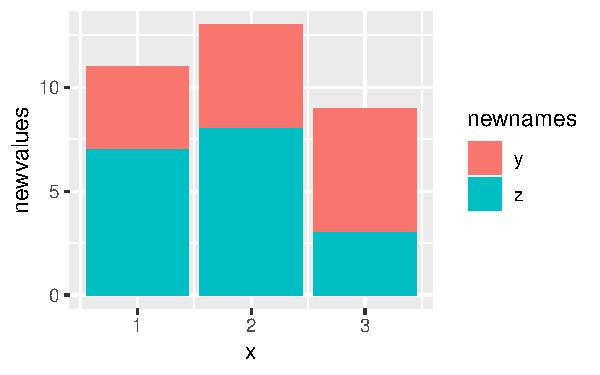
\includegraphics{bar-charts-in-ggplot-with-multiple-outcomes_files/figure-latex/unnamed-chunk-4-1}

\hypertarget{geom_col}{%
\subsubsection{\texorpdfstring{\texttt{geom\_col()}}{geom\_col()}}\label{geom_col}}

By default, \texttt{geom\_col()} assumes
\texttt{stat\ =\ \textquotesingle{}identity\textquotesingle{}}
i.e.~\texttt{y} is the height of the bar.

\begin{Shaded}
\begin{Highlighting}[]
\FunctionTok{ggplot}\NormalTok{(myReshapedData, }\CommentTok{\# data I am using}
       \FunctionTok{aes}\NormalTok{(}\AttributeTok{x =}\NormalTok{ x, }\CommentTok{\# x is newnames}
           \AttributeTok{y =}\NormalTok{ newvalues, }\CommentTok{\# y is newvalues}
           \AttributeTok{fill =}\NormalTok{ newnames)) }\SpecialCharTok{+} \CommentTok{\# fill is newnames}
  \FunctionTok{geom\_col}\NormalTok{() }\CommentTok{\# y is actual bar height}
\end{Highlighting}
\end{Shaded}

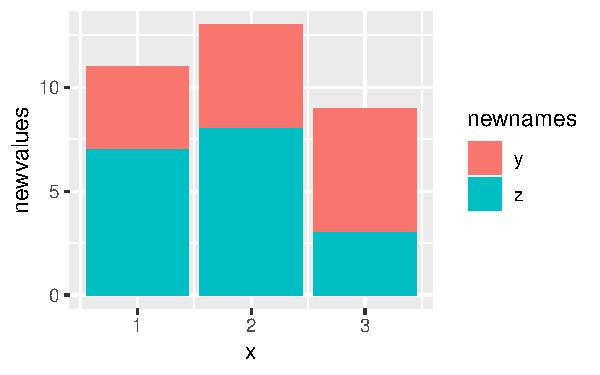
\includegraphics{bar-charts-in-ggplot-with-multiple-outcomes_files/figure-latex/unnamed-chunk-5-1}

\hypertarget{bar-chart-with-unstacked-bars}{%
\subsection{Bar Chart With Unstacked
Bars}\label{bar-chart-with-unstacked-bars}}

\begin{Shaded}
\begin{Highlighting}[]
\FunctionTok{ggplot}\NormalTok{(myReshapedData, }\CommentTok{\# data I am using}
       \FunctionTok{aes}\NormalTok{(}\AttributeTok{x =}\NormalTok{ x, }\CommentTok{\# x is newnames}
           \AttributeTok{y =}\NormalTok{ newvalues, }\CommentTok{\# y is newvalues}
           \AttributeTok{fill =}\NormalTok{ newnames)) }\SpecialCharTok{+} \CommentTok{\# fill is newnames}
  \FunctionTok{geom\_bar}\NormalTok{(}\AttributeTok{stat =} \StringTok{"identity"}\NormalTok{, }\CommentTok{\# y is actual bar height}
           \AttributeTok{position =} \FunctionTok{position\_dodge}\NormalTok{()) }\CommentTok{\# unstack bars}
\end{Highlighting}
\end{Shaded}

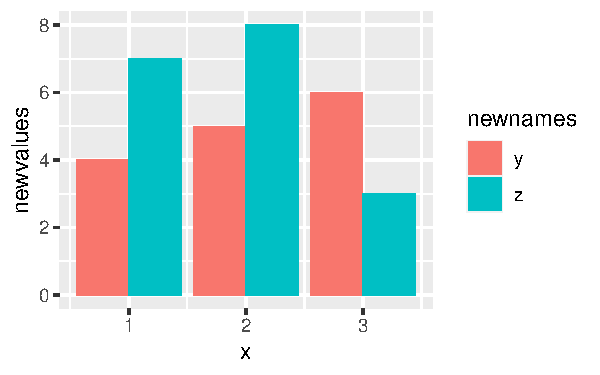
\includegraphics{bar-charts-in-ggplot-with-multiple-outcomes_files/figure-latex/unnamed-chunk-6-1}

\hypertarget{line-chart}{%
\subsection{Line Chart}\label{line-chart}}

\begin{Shaded}
\begin{Highlighting}[]
\FunctionTok{ggplot}\NormalTok{(myReshapedData, }\CommentTok{\# data I am using}
       \FunctionTok{aes}\NormalTok{(}\AttributeTok{x =}\NormalTok{ x, }\CommentTok{\# x is x}
           \AttributeTok{y =}\NormalTok{ newvalues, }\CommentTok{\# y is value}
           \AttributeTok{color =}\NormalTok{ newnames, }\CommentTok{\# color is key}
           \AttributeTok{group =}\NormalTok{ newnames)) }\SpecialCharTok{+} \CommentTok{\# line needs a group aesthetic}
  \FunctionTok{geom\_line}\NormalTok{()}
\end{Highlighting}
\end{Shaded}

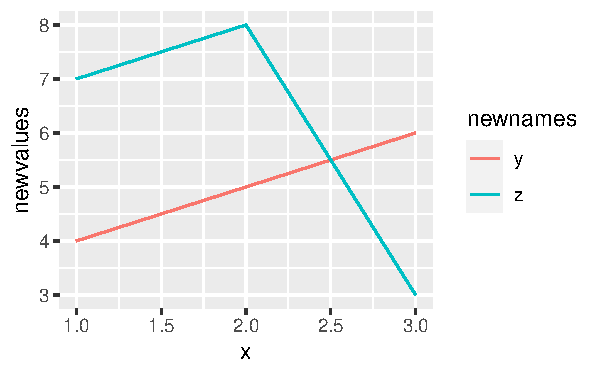
\includegraphics{bar-charts-in-ggplot-with-multiple-outcomes_files/figure-latex/unnamed-chunk-7-1}



\end{document}
